\documentclass{article}
\usepackage{amsmath,amsfonts,amsthm,amssymb,amsopn,bm}
\usepackage[margin=.9in]{geometry}
\usepackage{graphicx}
\usepackage{url}
\usepackage[usenames,dvipsnames]{color}
\usepackage{fancyhdr}
\usepackage{multirow}
\usepackage{listings}
\usepackage{hyperref}

\definecolor{keywords}{RGB}{255,0,90}
\definecolor{comments}{RGB}{0,0,113}
\definecolor{red}{RGB}{160,0,0}
\definecolor{green}{RGB}{0,150,0}
 
\lstset{language=Python, 
        basicstyle=\ttfamily\tiny, 
        keywordstyle=\color{keywords},
        commentstyle=\color{comments},
        stringstyle=\color{red},
        showstringspaces=false}

\newcommand{\argmax}{\arg\!\max}
\newcommand{\argmin}{\arg\!\min}
\newcommand{\field}[1]{\mathbb{#1}}
\newcommand{\1}{\mathbf{1}}
\newcommand{\E}{\mathbb{E}} 
\renewcommand{\P}{\mathbb{P}}
\newcommand{\N}{\mathcal{N}} % NormalDist
\newcommand{\R}{\field{R}} % real domain
% \newcommand{\C}{\field{C}} % complex domain
\newcommand{\F}{\field{F}} % functional domain
\newcommand{\T}{^{\textrm T}} % transpose
\def\diag{\text{diag}}

%% operator in linear algebra, functional analysis
\newcommand{\inner}[2]{#1\cdot #2}
\newcommand{\norm}[1]{\left\|#1\right\|}
\newcommand{\twonorm}[1]{\|#1\|_2^2}
% operator in functios, maps such as M: domain1 --> domain 2
\newcommand{\Map}[1]{\mathcal{#1}}
\renewcommand{\theenumi}{\alph{enumi}} 

\newcommand{\Perp}{\perp \! \! \! \perp}

\newcommand\independent{\protect\mathpalette{\protect\independenT}{\perp}}
\def\independenT#1#2{\mathrel{\rlap{$#1#2$}\mkern2mu{#1#2}}}
\newcommand{\vct}[1]{\boldsymbol{#1}} % vector
\newcommand{\mat}[1]{\boldsymbol{#1}} % matrix
\newcommand{\cst}[1]{\mathsf{#1}} % constant
\newcommand{\ProbOpr}[1]{\mathbb{#1}}
\newcommand{\points}[1]{\small\textcolor{magenta}{\emph{[#1 points]}} \normalsize}
\date{{}}

\setlength\parindent{0px}

\begin{document}
\title{Homework \#1 A}
\author{\normalsize{Spring 2020, CSE 446/546: Machine Learning}\\
\normalsize{Dino Bektesevic}}
\maketitle

Collaborated: Conor Sayers, Joachim Moeyenes, Jessica Birky, Leah Fulmer

\section*{Conceptual Questions \points{10} }
The answers to these questions should be answerable without referring to external materials.  Briefly justify your answers with a few words.
\begin{enumerate}
    \item \points{2} Suppose that your estimated model for predicting house prices has a large positive weight on ’number of bathrooms’. Does it implies that if we remove the feature ”number of bathrooms” and refit the model, the new predictions will be strictly worse than before?  Why?\\
    If number of bathrooms is independent feature our predictions would be worse. But as we discussed in class, often it is hte case that number of bathrooms is really not an independent feature in the feature set, but instead the weights are split between several different factors that directly or indirectly measure the number of bathrooms. 
        
    \item \points{2} Compared to L2 norm penalty, explain why a L1 norm penalty is more likely to result in a larger number of 0s in the weight vector or not?\\
    L1 norm is the sum of the lengths of the projections of the vector components onto the coordinate axes. For example take a point $(1, 1)$. The L1 norm of that point is 2, while the L2 norm of that point is the, more commonly expected vector magnitude, $\sqrt2$. For the same vector magnitude, vector's L2 norm, L1 will claim point $(\sqrt 2, 0)$ is closer than point $(1, 1)$. L1 penalty will therefore penalize those points that are "more aligned" to the basis vectors of the space we're in. For a lack of a better way to verbalize this: penalizing using L1 norm produces sparser outputs because L1 norm awards points that can be expressed using smaller number of basis vectors. Basis vectors themselves are sparse and if we can force using less of them, the end weights will be expressible by using a smaller number of basis vectors, i.e. weights will have more zeros in them.
        
    \item \points{2} In at most one sentence each, state one possible upside and one possible downside of using the following regularizer: $\sum_i|w_i|^{0.5})$ \\
    All these regularizers belong a different $L_p$ norms, where for $p=2$ we have Euclidian distance, $p=1$ the taxicab distance, $p=0$ the count of non-zero vector components, each producing a sparser solution than the previous one. \\
    But the point of regularization is to restrict weight values to smaller values and the square root diverges closer to zero we get, which is exactly the opposite of what we want.
        
    \item \points{1} True or False:  If the step-size for gradient descent is too large, it may not converge. \\
    True. When jumps occur with a step-size much greater than the characteristic step length of a function we can end up constantly jumping to higher values and further away from the minimum.
    
    \item \points{2} In your own words, describe why SGD works. \\
    Gradient descent effectively works by starting from a random point and then calculating gradient at that point with respect to all features in the dataset in order to pick the direction of the next point it will step to. Computing true gradients of the sum of squared residuals with respect to features is very costly with datasets containing a lot of points for even moderate number of features. Stochastic gradient descent computes the gradient using a randomly selected point, or a set of points, instead of computing the true gradient using all points. This obviously works for relatively monotonic functions since what we have effectively done was approximating the true function with a line or a hyperplane.
    
    \item \points{2}In at most one sentence each, state one possible advantage of SGD (stochastic gradient descent)over GD (gradient descent) and one possible disadvantage of SGD relative to GD. \\
    SGD is much less computationally demanding, but might take a longer time to converge to minimum value than GD might. GD on the other hand virtually guarantees that fewer steps will need to be taken to converge to minimum compared to SGD.
    \end{enumerate}





\section*{Convexity and Norms \points{10}}
A.1. A norm $||\cdot||$ over $R^n$ is defined by the properties:
\begin{enumerate}
\item[] \begin{enumerate}
    \item non-negative: $||x||\ge 0 \forall x \in \R^n \iff x= 0$,
    \item absolute scalability: $||ax|| = |a| ||x|| \forall a \in \R$  and $x\in\R^n$,
    \item triangle inequality: $||x+y|| \le ||x|| + ||y|| \forall x,y \in \R^n$
\end{enumerate}

\item Show that $f(x) = (\sum^n_{i=1}|x_i|)$ is a norm. (Hint: begin by showing that $|a+b| \leq |a|+|b| \forall a,b \in \R$. \\
Trick is to notice that norm is defined over a field we are very familiar with and which rules we know. Since $x_i\in\R \rightarrow |x_i|\geq 0$ by definition of absolute value of a number we can write:
$$f(\vec x) = ||\vec x|| = \sum |x_i| \geq 0$$
We show absolute homogeneity using same trick:
$$f(a\vec x)= ||a\vec x|| = \sum |ax_i| = \sum |a||x_i| = |a|\sum|x_i| = |a|||\vec x|| = |a|f(x)$$
where first we applied the norm we are testing, wrote out its definition, found ourselves operating on elements of $\R$ where associativity and multiplicativity applies, rewrote so it suits our purpose, and then walked back up the chain. Triangle inequality is likely the most interesting property to prove. Question requires us to prove the triangle inequality in $\R$ first. For any $a,b\in\R$ from definition of absolute value it follows:
\begin{align*}
\centering
    -|a|\leq a &\leq |a| \\
    -|b|\leq b &\leq |b|
\end{align*}
Summing the first two rows we have 
$$-(|a|+|b|)\leq a + b \leq |a| + |b| $$
Since $|c|\leq d \rightarrow -d \leq c \leq d$, we identify $c:=a+b$ and $d:=|a|+|b|$ we rewrite the line above as:
$$|a+b|\leq |a|+|b|$$
This proof is effectively a clearer more verbose version of Wikipedia proof. It's hard to find yet another way to prove triangle inequality. Applying the triangle relativity in $\R$ to our problem:
\begin{align*}
    f(\vec x + \vec y) &= ||\vec x + \vec y|| = \sum |x_i + y_i| \\
    & \leq \sum \left( |x_i| + |y_i|\right) \\
    &= \sum |x_i| + \sum |y_i| \\
    & = ||\vec x|| + ||\vec y|| = f(\vec x) + f(\vec y) \\
    \rightarrow f(\vec x + \vec y) &\leq f(\vec x) + f(\vec y) 
\end{align*}{}

\newpage
\item \points{2} Show that $g(x) =(\sum^n_{i=1}|x_i|^{1/2})^2$ is not a norm. (Hint: it suffices to find two points in $n= 2$ dimensions such that the triangle inequality does not hold.) \\
Since:
\begin{align*}
    (\sqrt{|x_i|} + \sqrt{|y_i|})^2 &= |x_i| + |y_i| + 2\sqrt{|x_i||y_i|} \geq |x_i| + |y_i| \\
    (\sqrt{|x_i|} + \sqrt{|y_i|})^2 &\geq |x_i| + |y_i| \\
    \sqrt{|x_i|} + \sqrt{|y_i|} &\geq \sqrt{|x_i| + |y_i|}
\end{align*}
Applying the norm definition and the inequality shown above:
\begin{align*}
    g(\vec x + \vec y) &= \sum \sqrt{|x_i + y_i|}^2 \\
    &\leq \sum (\sqrt{|x_i|+|y_i|})^2 \\
    &\leq \sum (\sqrt{|x_i|}+\sqrt{|y_i|})^2 \\
    g(\vec x + \vec y) &\leq \sum \left(|x_i| + |y_i| + 2\sqrt{|x_i||y_i|}\right) \\
    g(\vec x + \vec y) &\leq g(\vec x) + g(\vec y) + 2\sum\sqrt{|x_i||y_i|}
\end{align*}
Therefore it's not clear that the triangle inequality holds. 

\end{enumerate}

Context: norms are often used in regularization to encourage specific behaviors of solutions. If we define $||x||_p:= (\sum^n_i = \1|x_i|^p)^{1/p}$ then one can show that $||x||^p$ is a norm for all $p\ge1$. The important cases of $p=2$ and $p=1$ correspond to the penalty for ridge regression and the lasso, respectively.


\vskip 2cm
A 2.\points{3} A set $A\subseteq \R^n$ is convex if $\lambda x + (1-\lambda)y \in A \forall x,y \in A$ and $\lambda\in [0,1]$. For each of the grey-shaded sets (I-III), state whether each one is convex, or state why it is not convex using any of the points a,b,c,d in your answer.\\
I is not convex because we exit the image if we connect b and c. \\
II is convex, there are no combinations of points that would exit the image. \\
III is not convex because it is possible to connect points d and a in a way that exists the image.




\vskip 2cm
A 3.\points{4} We say a function $f:\R^d\rightarrow\R$ is convex on a set $A \iff (\lambda x + (1-\lambda)y)\leq \lambda f(x) + (1-\lambda)f(y) \forall x,y \in A$ and $\lambda\in [0,1]$. For each of the grey-colored functions (I-III), state whether each one is convex on the given interval or state why not with a counter example using any of the points a,b,c,d in your answer

\begin{enumerate}
    \item Function in panel I on [a,c]: Function is convex as there are no points that exit the graph.
    \item Function in panel II on [a,c]: Function is not convex as it's possible to connect b and c such that we exit the graph.
    \item Function in panel III on [a,d]: Connecting f(a) to f(d) exists the graph - not convex.
    \item Function in panel III on [c,d]: Connecting f(c) to f(d) does not exit the graph, - convex in that interval.
\end{enumerate}{}




\newpage 
\section*{Lasso \points{45}}
Given $\lambda > 0$ and data $(x_1,y_1),...,(x_n,y_n)$, the Lasso is the problem of solving 
$$\argmin_{w\in\R^d,b\in\R^n} \sum_{i=1}^n (x^T_i w + b - y_i)^2 + \lambda\sum^d_{j=1}|w_j|$$
$\lambda$ is a regularization tuning parameter. For the programming part of this homework, you are required to implement the coordinate descent method of Algorithm 1 that can solve the Lasso problem. You may use common computing packages (such as NumPy or SciPy), but do not use an existing Lasso solver (e.g., of scikit-learn). 


A4. We will first try out your solver with some synthetic data. A benefit of the Lasso is that if we believe many features are irrelevant for predicting $y$, the Lasso can be used to enforce a sparse solution, effectively differentiating between the relevant and irrelevant features. Suppose that $x\in\R^d, y\in\R,k < d$, and pairs of data $(x_i,y_i)$ for $i= 1,\hdots n$ are generated independently according to the model $y_i= w^Tx_i +\epsilon_i$ where
$$h(z) = \begin{cases} 
    j/k &\mbox{if } j \in \{1, \hdots ,k\} \\
    0 &\mbox{otherwise }  \\
\end{cases} 
$$ 
where $\epsilon_i \approx \N(0,\sigma^2)$ is some Gaussian noise (in the model above $b=0$). Note that since $k < d$, the features $k+1$ through $d$ are unnecessary (and potentially even harmful) for predicting $y$. With this model in mind, let $n= 500,d= 1000,k= 100$, and $\sigma=1$. Generate some data by choosing $x_i\in\R^d$, where each component is drawn from a $\N(0,1)$ distribution and $y_i$ generated as specified above. 
\begin{enumerate}
    \item \points{10} With your synthetic data, solve multiple Lasso problems on a regularization path, starting at $\lambda_{\max}$ where 0 features are selected and decreasing $\lambda$ by a constant ratio (e.g., 1.5) until nearly all the features are chosen. In plot 1, plot the number of non-zeros as a function of $\lambda$ on the x-axis (Tip: use log scale).
    \item \points{10} For each value of $\lambda$ tried, record values for false discovery rate (FDR) (number of incorrect non zeros in $\widehat w/$total number of non zeros in $\widehat w$) and true positive rate (TPR) (number of correct non zeros in $\widehat w/k$). In plot 2, plot these values with the x-axis as FDR, and the y-axis as TPR and note that in an ideal situation we would have an (FDR,TPR) pair in the upper left corner, but that can always trivially achieve $(0,0)$ and $(d-kd,1)$. \\
    For both a and b parts of the problem we have the following graph:
    \begin{figure}[h!]
        \centering
        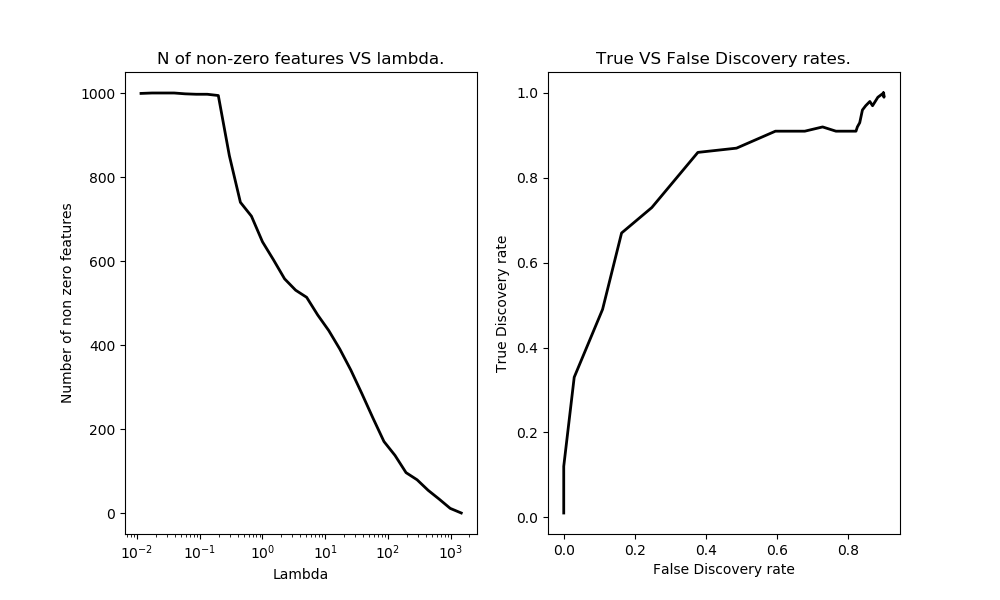
\includegraphics[width=0.8\textwidth]{HW2/HW2_plots/CoordinateDescent.png}
    \end{figure}
    
    \newpage
    \item \points{5} Comment on the effect of $\lambda$ in these two plots. \\
    No features are selected in the first step, i.e. close to $\lambda_{\max}$. Successive iterations relax regularization penalties so more and more features are selected. Simultaneously TPR increases very rapidly initially and then tapers off the rapid growth. This occurs because we quickly learn the most important features after which adding more features just doesn't add that much more valuable information to the model. Simultaneously our FDR skyrockets because the additional features over-specify our model. Eventually TPR jumps to nearly one as, I assume, we just fit all the points. \\

Figures provided by the following code:
 
\lstinputlisting[linerange={0-269,454-456}]{HW2_code_solutions/coordinate_descent.py}  
\end{enumerate}




\newpage
A5. Now we put the Lasso to work on some real data.  Download the training data set “crime-train.txt” and the test data set “crime-test.txt” from the website under Homework 2.  Store your data in your working directory and read in the files with:
\begin{lstlisting}[language=Python]
import pandas as pd
df_train = pd.read_table("crime-train.txt")
df_test = pd.read_table("crime-test.txt")
\end{lstlisting}

The data consist of local crime statistics for 1,994 US communities. The response $y$ is the crime rate. The name of the response variable isViolentCrimesPerPop, and it is held in the first column of df\_train and df\_test. There are 95 features. These features include possibly relevant variables such as the size of the police force or the percentage of children that graduate high school. The data have been split for you into a training and test set with 1,595 and 399 entries, respectively.

We’d like to use this training set to fit a model which can predict the crime rate in new communities and evaluate model performance on the test set. As there are a considerable number of input variables, over fitting is a serious issue. In order to avoid this, use the coordinate descent LASSO algorithm you just implemented in the previous problem. Begin by running the LASSO solver with $\lambda = \lambda_{\max}$ defined above. For the initial weights, just use 0. Then, cut $\lambda$ down by a factor of 2 and run again, but this time pass in the values of $\widehat w$ from your $\lambda = \lambda_{\max}$ solution as your initial weights. This is faster than initializing with 0 weights each time. Continue the process of cutting $\lambda$ by a factor of 2 until the smallest value of $\lambda$ is less than 0.01. For all plots use a log-scale for the $\lambda$d dimension.

\begin{enumerate}
    \item \points{4} Plot the number of nonzeros of each solution versus $\lambda$ \\
    \begin{figure}[h!]
        \centering
        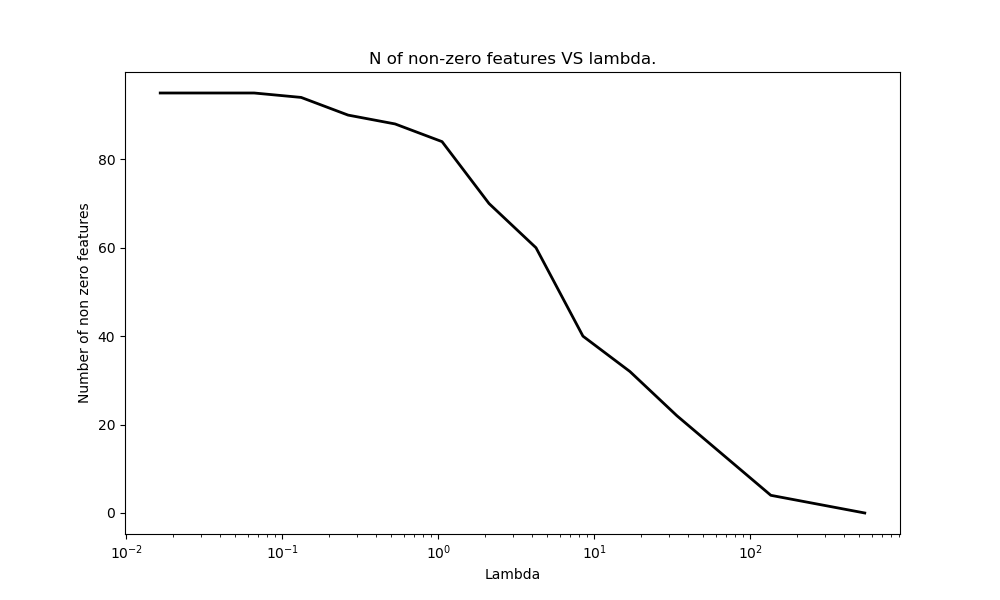
\includegraphics[width=0.6\textwidth]{HW2/HW2_plots/A5ZerosVSLambdas.png}
    \end{figure}

    \newpage
    \item \points{4} Plot the regularization paths (in one plot) for the coefficients for input variables agePct12t29, pctWSocSec, pctUrban, agePct65up, and householdsize. \\ 
    
    \begin{figure}[h!]
        \centering
        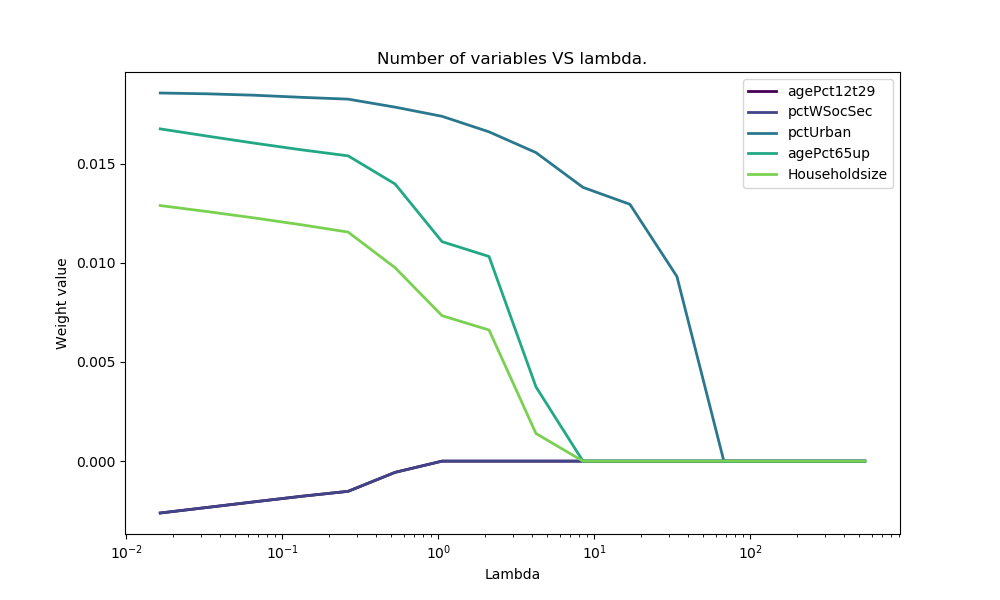
\includegraphics[width=0.6\textwidth]{HW2/HW2_plots/5RegPaths.png}
    \end{figure}
    
    \item \points{4} Plot the squared error on the training and test data versus $\lambda$ \\
    \begin{figure}[h!]
        \centering
        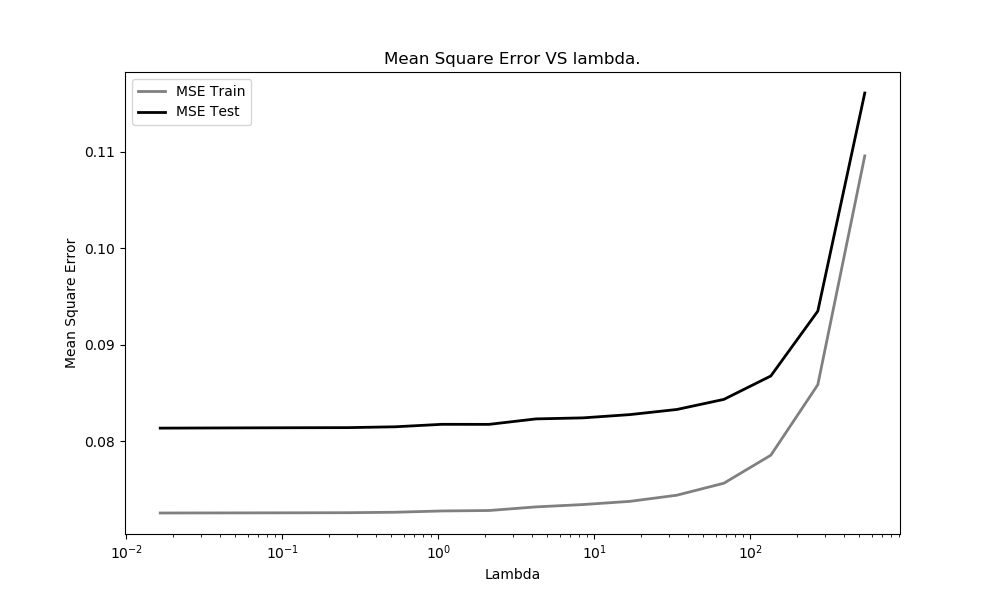
\includegraphics[width=0.6\textwidth]{HW2/HW2_plots/MSEA5.png}
    \end{figure}
    
    \newpage
    \item \points{4} Sometimes a larger value of $\lambda$ performs nearly as well as a smaller value, but a larger value will select fewer variables and perhaps be more interpretable. Inspect the weights (on features) for $\lambda = 30$. Which feature variable had the largest (most positive) Lasso coefficient? What about the most negative? Discuss briefly. A description of the variables in the data set can be found here: \url{http://archive.ics.uci.edu/ml/machine-learning-databases/communities/communities.names}. \\
    
    Maximal value of $w=0.0680$ belongs to feature PctIlleg. PctIlleg is percentage of kids born to never married persons indicative of unstable home life and lack of support system. Following with the next highest weights we can see that percentage of persons living in dense housing (more than 1 person per room), number of vacant households and number of homeless people counted on the streets also highly correlate with total number of violent crimes. This indicates that violent crimes tend to be more common in poorer areas, with poor living conditions. This is telling us that is still possible to be unmarried with a kid, or a kid with unmarried parents, without committing a violent crime, as correlation is not necessarily causation.  \\
    Minimal value of $w=-0.0702$ belongs to feature PctKids2Par. PctKids2Par is percentage of kids in family housing with two parents. The feature is indicative of stable home life, an existence of support system, both financial and emotional, for the child so it does not come as a surprise it anti-correlates with the total number of violent crimes per 100 000 population. 

    \begin{table}[h!]
    \centering
        \begin{tabular}{l|c}
        \centering
            Feature Name              &  Magnitude \\
            \hline
            PctKids2Par               & -0.07017508 \\
            PctHousOccup              & -0.00724790 \\
            PctWorkMom                & -0.00544586 \\
            agePct12t29               & -0.00367240 \\
            LemasPctOfficDrugUn       & 0.00051549 \\
            PctVacantBoarded          & 0.00126885 \\
            pctUrban                  & 0.01042646 \\
            MalePctDivorce            & 0.01102267 \\
            NumStreet                 & 0.01575945 \\
            HousVacant                & 0.02049849 \\
            PctPersDenseHous          & 0.03062536 \\
            PctIlleg                  & 0.06802481 
        \end{tabular}{}
    \end{table}{}

    
    \item \points{4} Suppose there was a large negative weight on agePct65up and upon seeing this result, a politician suggests policies that encourage people over the age of 65 to move to high crime areas in an effort to reduce crime. What is the (statistical) flaw in this line of reasoning? (Hint:  fire trucks are often seen around burning buildings, do fire trucks cause fire?) \\
    As mentioned above correlation is not necessarily causation. Moving elderly into violent crime areas would likely reduce some crime statistics that are not population-corrected but overall would not have a profound effect on crime, except perhaps providing criminals with easier-to-assault targets. That said, I have never seen a fire start but I have often seen fire trucks suspiciously close to one, so who knows. 
    
    
\newpage
\lstinputlisting[linerange={0-148,309-455,457-}]{HW2_code_solutions/coordinate_descent.py}
\end{enumerate}



\newpage
\section*{Binary Logistic Regression \points{30}}
A6. Let us again consider the MNIST dataset, but now just binary classification, specifically, recognizing if a digit is a 2 or 7. Here, let Y= 1 for all the 7’s digits in the dataset, and use Y=-1 for 2. We will use regularized logistic regression.  Given a binary classification dataset ${(x_i,y_i)}^n_{i=1}$ for $x_i\in\R$ dand $y_i\in {-1,1}$ we showed in class that the regularized negative log likelihood objective function can be written a
$$J(w,b) = \frac{1}{n} \sum_{i=1}^n \log{\left( 1 + e^{-y_i(b+x^T_iw)} \right)} + \lambda||w||^2_2$$
Note that the offset term $b$ is not regularized. For all experiments, use $\lambda = 10^{-1}$. Let $\mu_i(w,b) = \frac{1}{1+exp(-y_i(b+x^T_iw))}$
\begin{enumerate}
    \item \points{8} Derive the gradients $\nabla_wJ(w,b)$, $\nabla_bJ(w,b)$ and give your answers in terms of $\mu_i(w,b)$  (your answers should not contain exponentials). \\
    Write $J$ over $\mu$ to get a more general expression:
    \begin{align*}
        \nabla_w J(w,b) &= \nabla_w \frac{1}{n} \sum_{i=1}^n \log{\left( 1 + e^{-y_i(b+x^T_iw)} \right)} + \lambda||w||^2_2 \\
        &= \frac{1}{n} \sum_{i=1}^n \nabla_w \left(\log{\frac{1}{\mu_i(w,b)}} + \lambda||w||^2_2\right) \\
        &= \frac{1}{n} \sum_{i=1}^n \frac{-1}{\mu_i(w,b)\ln{10}} \nabla_w \mu_i(w,b) + 2\lambda w
    \end{align*}{}
    Solve $\nabla \mu_i$ for $w$ and $b$ via substitution and chain rule to get both required gradients:
    \begin{align*}
        \nabla_w \mu_i(w,b) &= \nabla_w \frac{1}{1+e^{-y_ib-y_ix^T_iw}} = \frac{-y_ix_i e^{-y_ib - y_ix^T_iw}}{-\left(1+e^{-y_ib - y_ix^T_iw}\right)^2} \\
        & = \left(y_ix_i e^{-y_ib - y_ix^T_iw} \right)\mu_i^2 = y_i x_i \left(\frac{1}{\mu_i} -1 \right)\mu_i^2 \\
        & = y_ix_i \mu_i(1-\mu_i)\\
        \nabla_b \mu_i(w,b) &= \nabla_b \frac{1}{1+e^{-y_ib-y_ix^T_iw}} = \frac{-y_i e^{-y_ib - y_ix^T_iw}}{-\left(1+e^{-y_ib - y_ix^T_iw}\right)^2} \\
        & = \left(y_i e^{-y_ib - y_ix^T_iw} \right)\mu_i^2 = y_i \left(\frac{1}{\mu_i} -1 \right)\mu_i^2 \\
        & = y_i \mu_i(1-\mu_i)
    \end{align*}{}
    Returning to $J$ we have:
    \begin{align*}
        \nabla_w J(w,b) &= \frac{-1}{n\ln{10}} \sum_{i=1}^n \frac{1}{\mu_i(w,b)} y_ix_i \mu_i(1-\mu_i) + 2\lambda w \\
        & = \frac{1}{n\ln{10}} \sum_{i=1}^n y_ix_i (\mu_i - 1) + 2\lambda w \\
        \nabla_b J(w,b) &= \frac{-1}{n\ln{10}} \sum_{i=1}^n \frac{1}{\mu_i(w,b)} y_i \mu_i(1-\mu_i) \\
        & = \frac{1}{n\ln{10}} \sum_{i=1}^n y_i (\mu_i - 1)
    \end{align*}{}
    
    
    \newpage
    \item \points{8} Implement gradient descent with an initial iterate of all zeros. Try several values of step sizes to find one that appears to make convergence on the training set as fast as possible. Run until you feel you are near to convergence.
    \begin{enumerate}
        \item For both the training set and the test, plot $J(w,b)$ as a function of the iteration number (and show both curves on the same plot) \\
        \begin{figure}[h!]
        \centering
            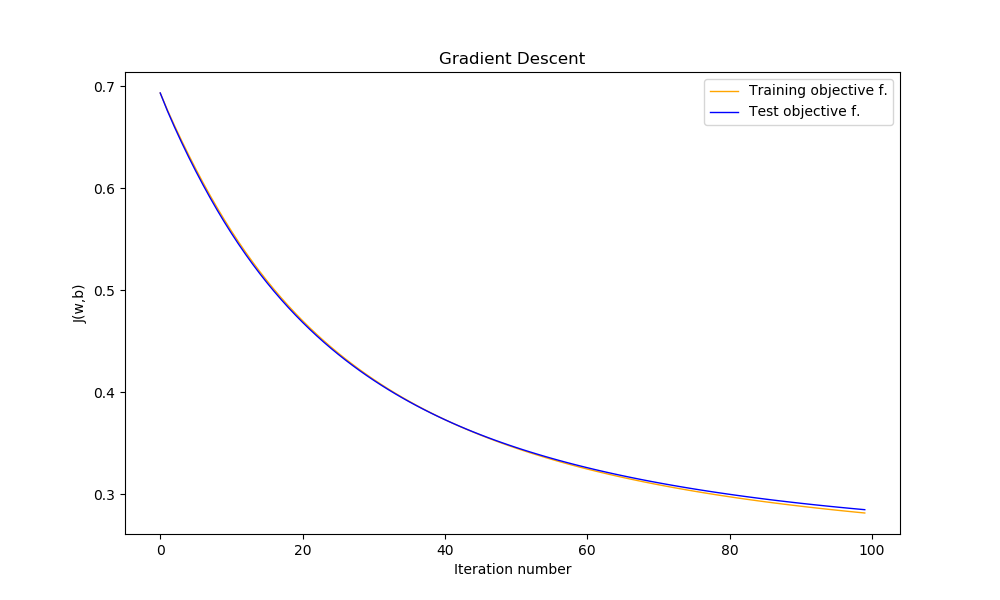
\includegraphics[width=0.6\textwidth]{HW2/HW2_plots/JwbA6b.png}
        \end{figure}
        \item For both the training set and the test, classify the points according to the rule $sign(b+x^T_iw)$ and plot the misclassification error as a function of the iteration number (and show both curves on the same plot). Note that you are only optimizing on the training set. The $J(w,b)$ and misclassification error plots should be on separate plots.
        \begin{figure}[h!]
        \centering
            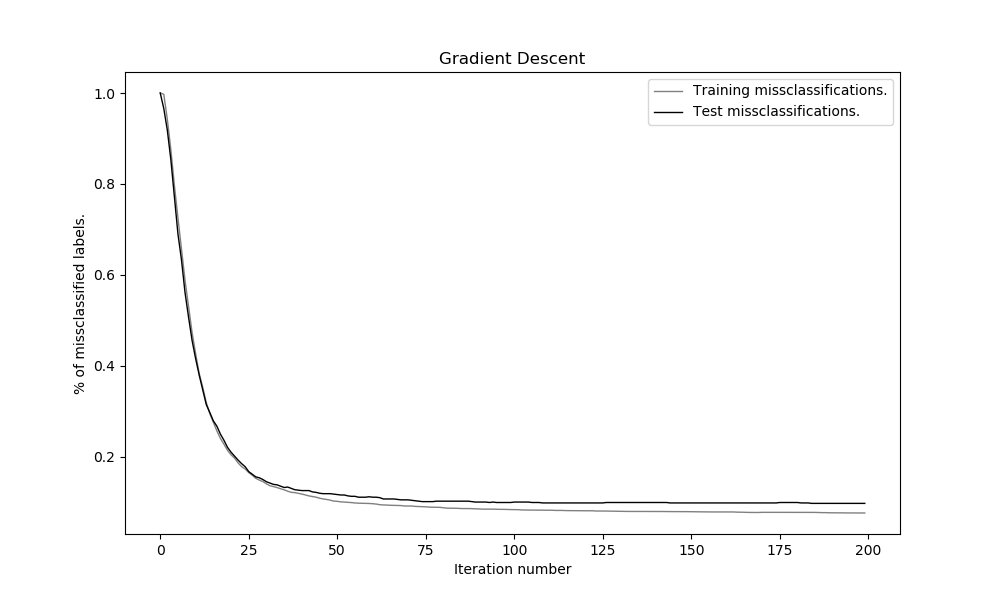
\includegraphics[width=0.6\textwidth]{HW2/HW2_plots/missclassificationsA6b.png}
        \end{figure}
    \end{enumerate}
    
    \newpage
    \item \points{7} Repeat (b) using stochastic gradient descent with a batch size of 1. Note, the expected gradient with respect to the random selection should be equal to the gradient found in part (a). Take careful note of how to scale the regularizer.
    
    \begin{figure}[h!]
    \centering
        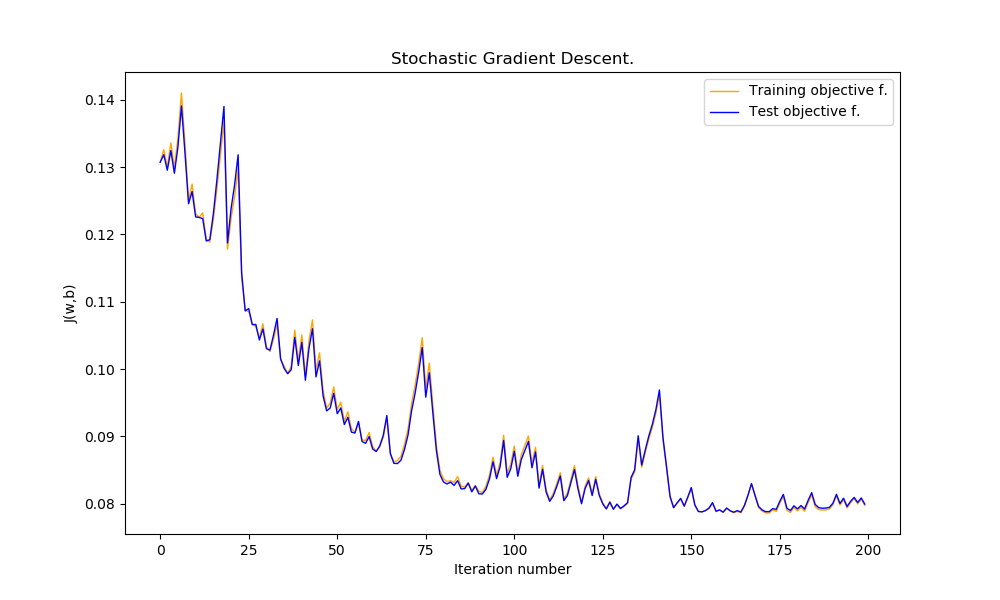
\includegraphics[width=0.6\textwidth]{HW2/HW2_plots/JwbA6c.png}
    \end{figure}
    
    \begin{figure}[h!]
    \centering
        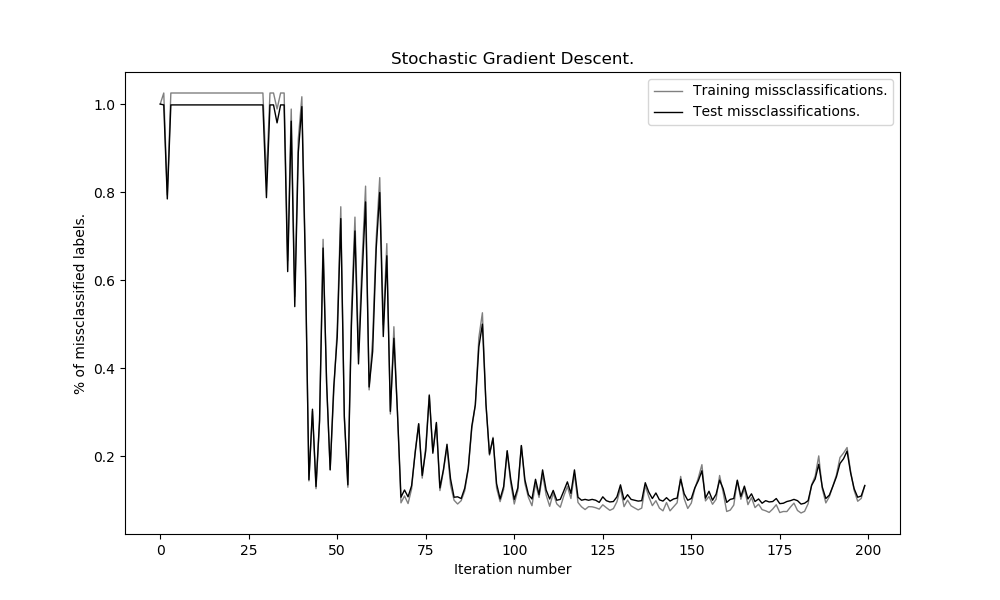
\includegraphics[width=0.6\textwidth]{HW2/HW2_plots/missclassificationsA6c.png}
    \end{figure}

    \newpage
    \item \points{7} Repeat (b) using stochastic gradient descent with batch size of 100. That is, instead of approximating the gradient with a single example, use 100. Note, the expected gradient with respect to the random selection should be equal to the gradient found in part (a).
    
    \begin{figure}[h!]
    \centering
        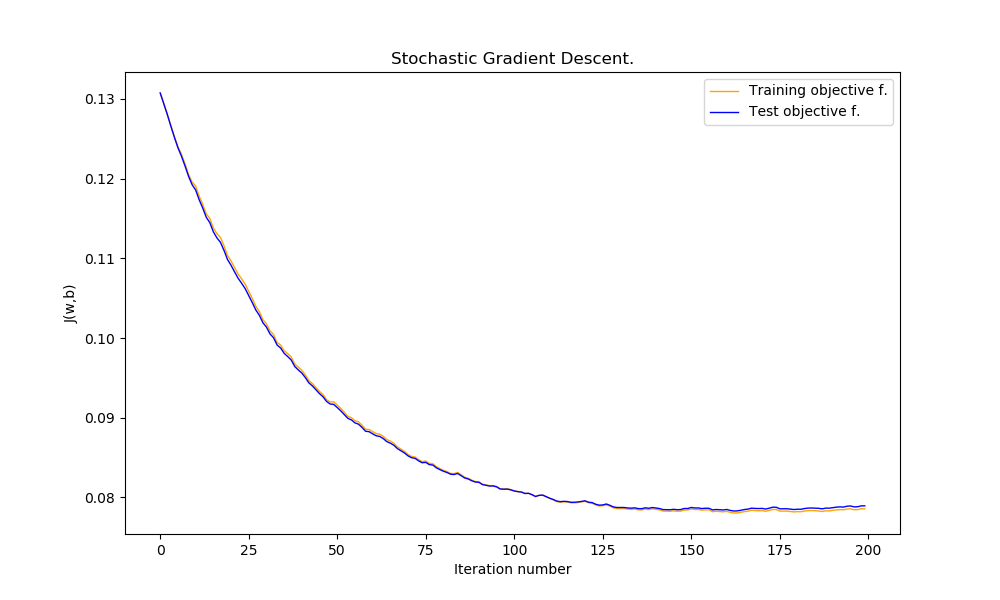
\includegraphics[width=0.6\textwidth]{HW2/HW2_plots/JwbA6d.png}
    \end{figure}
    
    \begin{figure}[h!]
    \centering
        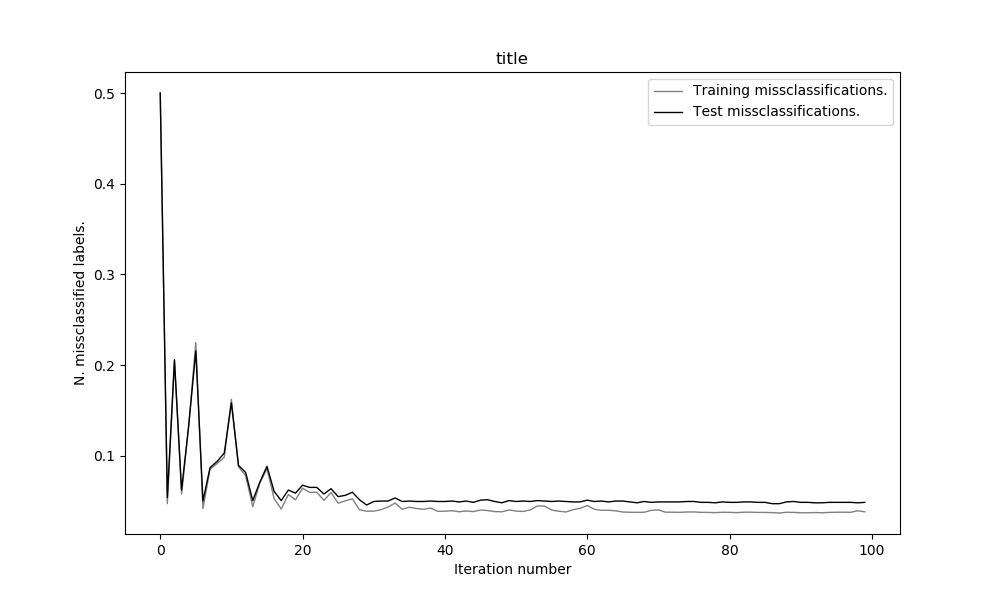
\includegraphics[width=0.6\textwidth]{HW2/HW2_plots/missclassificationsA6d.png}
    \end{figure}
\end{enumerate}

\newpage
\lstinputlisting[language=Python]{HW2_code_solutions/logistic_regression.py}



\end{document}
